\clearpage

\section{Fork}

\begin{tcolorbox}	
\begin{tabular}{p{2.75cm} p{0.2cm} p{10.5cm}} 	
\textbf{Header File}   &:& fork\_20171119.h \\
\textbf{Source File}   &:& fork\_20171119.cpp \\
\textbf{Version}       &:& 20171119 (\textbf{Student Name}: Romil Patel)
\end{tabular}
\end{tcolorbox}

\subsection*{Input Parameters}

--- NA ---

\subsection*{Input Signals}

\textbf{Number}: 1\\
\textbf{Type}: Any type (BinaryValue, IntegerValue, RealValue, ComplexValue, ComplexValueXY, PhotonValue, PhotonValueMP, Message)

\subsection*{Output Signals}

\textbf{Number}: 2\\
\textbf{Type}: Same as applied to the input.\\
\\
\textbf{Number}: 3\\
\textbf{Type}: Same as applied to the input.

\subsection*{Functional Description}

This block accepts any type signal and outputs two replicas of the input signal.

\begin{figure}[h]
	\centering
	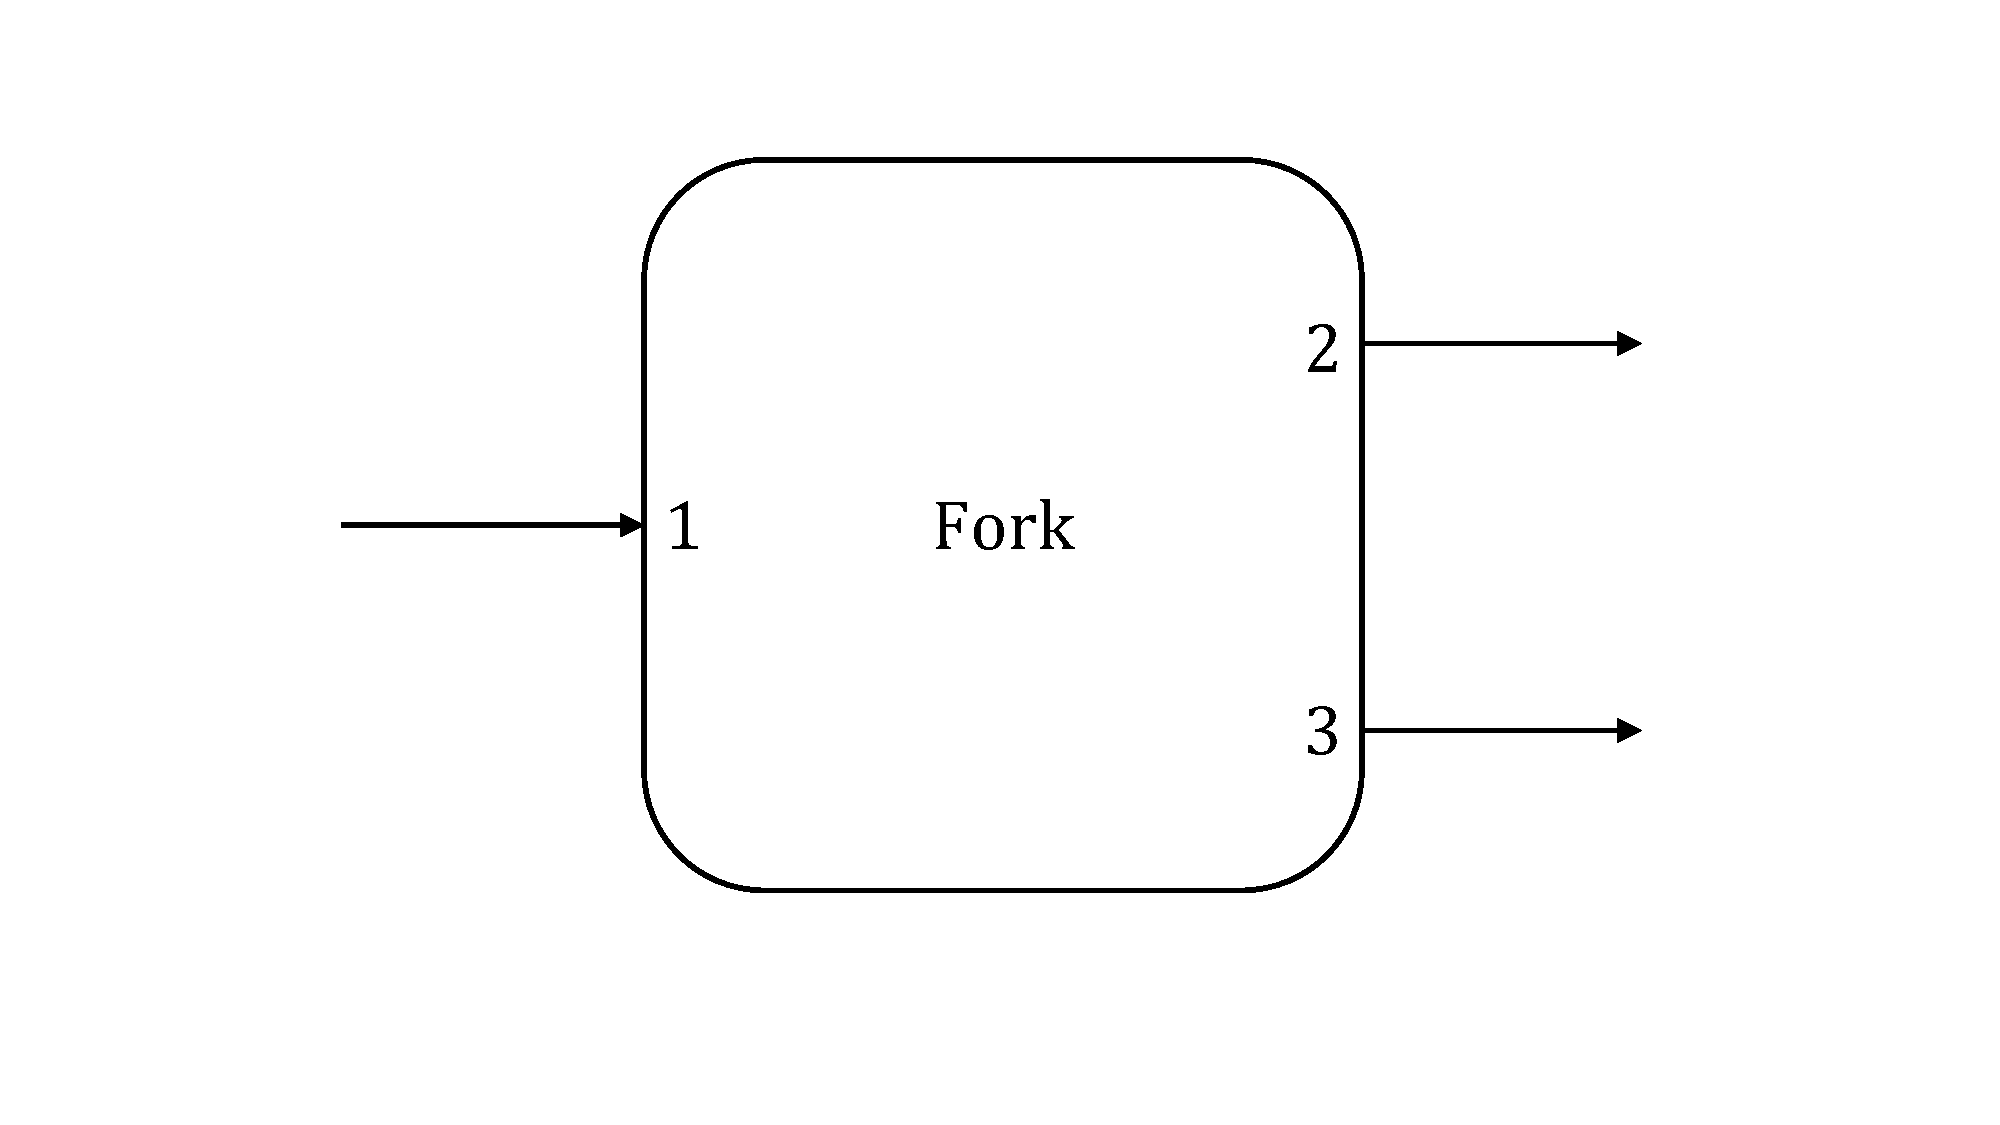
\includegraphics[width=0.6\textwidth, height=4.5cm]{./lib/fork/figures/fork.pdf}
	\caption{Fork}\label{}
\end{figure}